\begin{tikzpicture}
  \node[anchor=south east,inner sep=0] (pic_1) at (0,0) {
    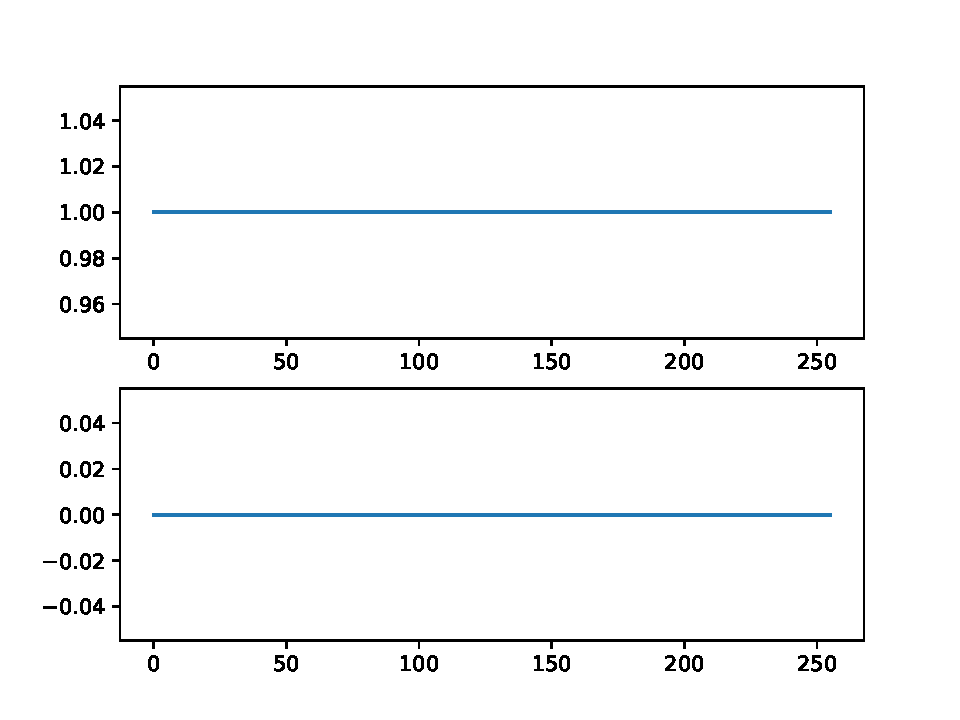
\includegraphics[width=0.5\linewidth]{diagrams/time_sync_combat_chan1.pdf}
  };

  \node[anchor=north east,inner sep=0] (pic_2) at (0,0) {
    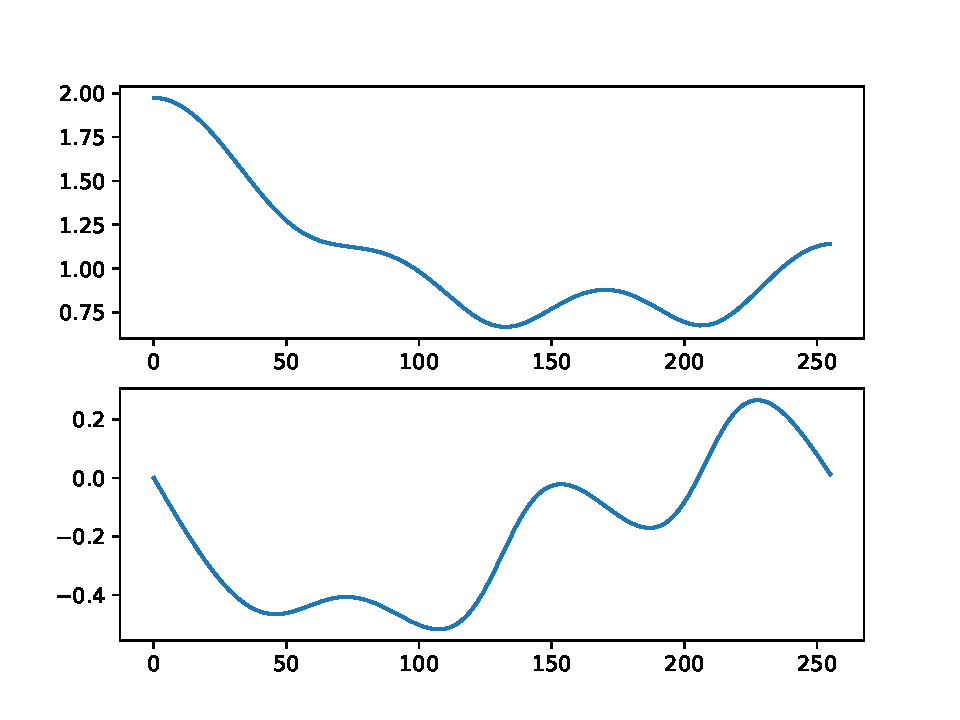
\includegraphics[width=0.5\linewidth]{diagrams/time_sync_combat_chan2.pdf}
  };

  \node[anchor=north west,inner sep=0] (pic_3) at (0,0) {
    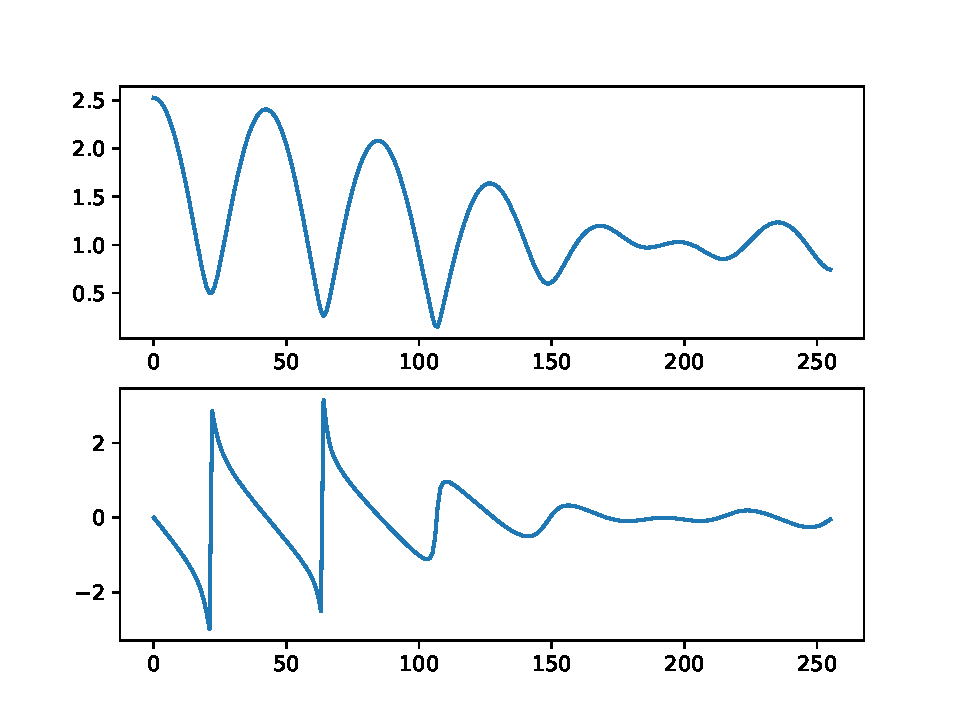
\includegraphics[width=0.5\linewidth]{diagrams/time_sync_combat_chan3.pdf}
  };

  \node[anchor=north east,inner sep=0] (pic_4) at (pic_2.south east) {
    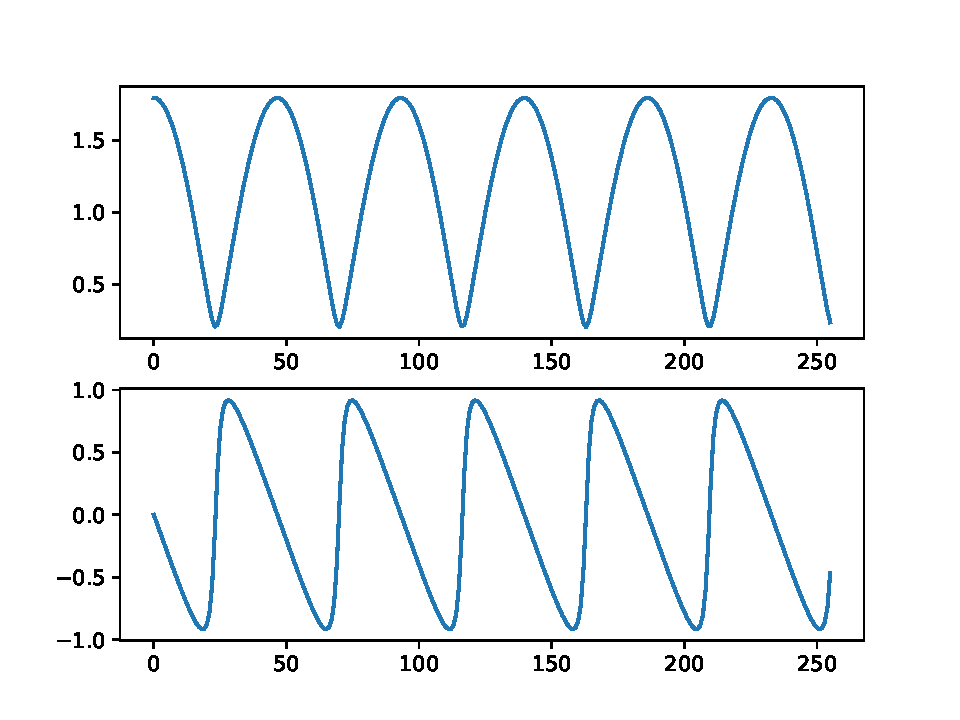
\includegraphics[width=0.5\linewidth]{diagrams/time_sync_combat_chan4.pdf}
  };

  \node[anchor=north west,inner sep=0] (pic_5) at (pic_3.south west) {
    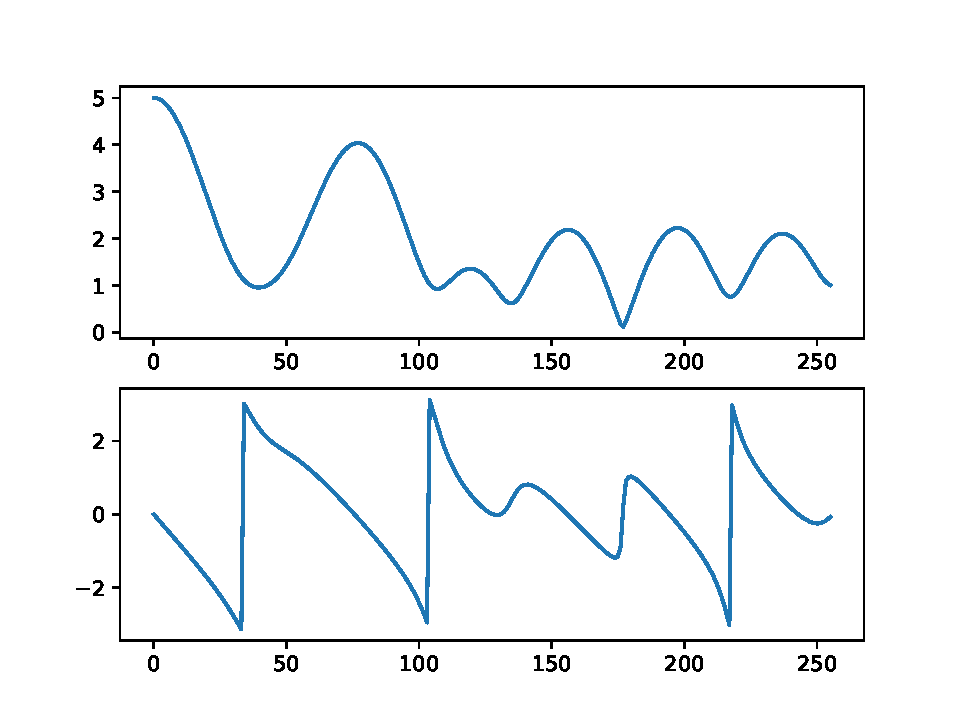
\includegraphics[width=0.5\linewidth]{diagrams/time_sync_combat_chan5.pdf}
  };

  \draw
  (pic_1.south) ++(0, 0.25) node[anchor=north]{\small{Channel 1}}
  (pic_2.south) ++(0, 0.25) node[anchor=north]{\small{Channel 2}}
  (pic_3.south) ++(0, 0.25) node[anchor=north]{\small{Channel 3}}
  (pic_4.south) ++(0, 0.25) node[anchor=north]{\small{Channel 4}}
  (pic_5.south) ++(0, 0.25) node[anchor=north]{\small{Channel 5}};

  \draw
  (pic_1.east) ++(-0.61,  0.94) -> ++(0.61, 0) node[anchor=west]{\small{Amplitude response}}
  (pic_1.east) ++(-0.61, -0.97) -> ++(0.61, 0) node[anchor=west]{\small{Phase response}};
\end{tikzpicture}
